\documentclass{article}
\usepackage{amsthm,amsmath,amsfonts,lipsum}
\usepackage[T1]{fontenc}
\usepackage{beramono}
\usepackage{listings}
\usepackage{fontawesome5}
\usepackage{adjustbox}
\usepackage{mathabx}
\usepackage{thmtools}
\usepackage{import}
\usepackage{graphicx}
\usepackage{setspace}
\usepackage{geometry}
\usepackage{physics}
\usepackage{float}
\usepackage[english]{babel}
\usepackage{framed}
\usepackage[dvipsnames,x11names]{xcolor}
\usepackage{tcolorbox}
\usepackage{fancyhdr}
\usepackage{hyperref}
\usepackage{booktabs}
\usepackage{enumitem}
\usepackage{cancel}
\usepackage{background}
\usepackage{units}

% Configuring the background
\backgroundsetup{
  scale=1, % Optional, scale if needed
  color=black, % Optional, set the image color, can be omitted
  opacity=0.18, % Optional, adjust opacity for watermark effect
  angle=0,
  position=current page.center, % Center the image on the page
  contents={
\includegraphics[width=1.75\paperwidth, height=1.75\paperheight, keepaspectratio]{ninym_ralei_leaf (watermarked by AlexanderTheMango)}} % Keeps aspect ratio and scales to fill the page
}

% Colours
\definecolor{darkgreen}{rgb}{0.0, 0.5, 0.0}
\definecolor{Firebrick}{rgb}{0.698, 0.132, 0.203}
\definecolor{Crimson}{rgb}{0.862745, 0.078431, 0.235294} % Crimson color
\definecolor{lightred}{rgb}{1.0, 0.819608, 0.819608} % Light red for background
\definecolor{MediumPurple}{rgb}{0.576, 0.439, 0.859}
\definecolor{chocolate}{rgb}{0.82, 0.41, 0.12} % Chocolate color definition
% Define the Navy color
\definecolor{Navy}{rgb}{0.0, 0.0, 0.5}

% Define custom tcolorbox styles for notes
\tcbuselibrary{skins, breakable}
\newtcolorbox{definitionbox}{colframe=RoyalBlue, colback=blue!5!white, title=Definition}
\newtcolorbox{examplebox}{colframe=ForestGreen, colback=green!5!white, title=Example}
\newtcolorbox{notebox}{colframe=RedOrange, colback=orange!5!white, title=Note}
\newtcolorbox{theorembox}{colframe=RoyalPurple, colback=purple!5!white, title=Theorem}

\newtcolorbox{propositionbox}{colframe=Goldenrod, colback=yellow!10!white, title=Proposition}
\newtcolorbox{remarkbox}{colframe=MidnightBlue, colback=blue!10!white, title=Remark}
\newtcolorbox{corollarybox}{colframe=OliveGreen, colback=green!10!white, title=Corollary}
\newtcolorbox{warningbox}{colframe=Crimson, colback=lightred, title=Warning}
\newtcolorbox{proofbox}{colframe=Black, colback=gray!10!white, title=Proof}
\newtcolorbox{questionbox}{colframe=Teal, colback=teal!10!white, title=Question}
\newtcolorbox{tipbox}{colframe=Goldenrod, colback=yellow!10!white, title=Tip}
\newtcolorbox{exercisebox}{colframe=darkgreen, colback=green!5!white, title=Exercise}
\newtcolorbox{solutionbox}{colframe=DodgerBlue4, colback=blue!5!white, title=Solution}
\newtcolorbox{algorithmbox}{colframe=Navy, colback=blue!10!white, title=Algorithm}
\newtcolorbox{conceptbox}{colframe=chocolate, colback=brown!10!white, title=Concept}
\newtcolorbox{illustrationbox}{colframe=Firebrick, colback=red!10!white, title=Illustration}
\newtcolorbox{intuitionbox}{colframe=MediumPurple, colback=purple!10!white, title=Intuition}
\newtcolorbox{answerbox}{colframe=RoyalBlue, colback=blue!10!white, title=Answer}

% Geometry settings
\geometry{letterpaper, portrait, includeheadfoot=true, hmargin=1in, vmargin=1in}
\onehalfspacing

% Header and footer
\pagestyle{fancy}
\fancyhf{}
\lhead{MAT232 - Lecture Notes}
\rhead{\thepage}
\lfoot{University of Toronto Mississauga}
\rfoot{\today}

% Document starts
\begin{document}
\renewcommand{\familydefault}{\rmdefault}

\begin{titlepage}
    \null % This is a TeX command that does nothing but is necessary for vfill to work correctly
    \vfill
    \begin{center}
        {\fontsize{40}{48}\selectfont \bfseries MAT232 - Lecture 13}
        \vspace{20pt} \\
        {\LARGE after partial derivatives?} \\
        \vspace{20pt}
        \textbf{AlexanderTheMango}
        \vspace{8pt}
        \\ Prepared for February 24, 2025
    \end{center}
    \vfill
\end{titlepage}


\setcounter{page}{0}
\newpage
\tableofcontents
\newpage

\begin{titlepage}
    \null % Ensures proper alignment with vfill
    \vfill
    \begin{center}
        {\Huge \textbf{Definitions and Theorems}} \\[20pt]
        \rule{\textwidth}{0.5mm} \\[15pt]
        {\Large \textit{Straight from the textbook — lots of fluff this time, more than what we need!}} \\[15pt]
        \rule{\textwidth}{0.5mm} \\[15pt]
        \textbf{Quick recap before diving into the lecture.}
    \end{center}
    \vfill
\end{titlepage}




\begin{titlepage}
    \null % Ensures proper alignment with vfill
    \vfill
    \begin{center}
        {\Huge \textbf{Let’s Get Started}} \\[20pt]
        \rule{\textwidth}{0.5mm} \\[15pt]
        {\Large \textit{Time to dive into the lecture notes.}} \\[15pt]
        \rule{\textwidth}{0.5mm} \\[15pt]
        \textbf{Grab your pen or pencil, and let’s break this down step by step.}
    \end{center}
    \vfill
\end{titlepage}

\normalsize

\setcounter{page}{1}

\section*{Review from the Previous Lecture}
\addcontentsline{toc}{section}{Review from the Previous Lecture}
\begin{remarkbox}
In the previous lecture, we covered important foundational concepts related to polar coordinates and their derivatives. Here’s a brief summary: 

\begin{itemize}
    \item \textbf{Derivative of \( r = f(\theta) \) in Cartesian Coordinates:}
    \large
    \[
        \dfrac{dy}{dx} = \dfrac{\dfrac{dy}{d\theta}}{\dfrac{dx}{d\theta}} = \dfrac{\dfrac{dr}{d\theta}\sin\theta + r\cos\theta}{\dfrac{dr}{d\theta}\cos\theta - r\sin\theta}
    \]
    \normalsize
    This formula helps us compute the slope of the tangent line for polar curves when converted to Cartesian coordinates. 

    \item \textbf{Equation of a Circle:}
    \[
        (x-h)^2 + (y-k)^2 = r^2
    \]
    Here:
    \begin{itemize}
        \item[\labelitemi] \( r \): Radius of the circle
        \item[\labelitemi] \( (h, k) \): Centre of the circle
    \end{itemize}    
\end{itemize}

\begin{notebox}
\textbf{Reminder:} Term Test 1 is scheduled for \textbf{Thursday, January 30th, 2025 (Week 4)}. Make sure to review polar derivatives, transformations, and conic sections!
\end{notebox}
\end{remarkbox}

\section*{Exploring Common Curve Shapes}
\addcontentsline{toc}{section}{Exploring Common Curve Shapes}

\subsection*{Parabola}
\addcontentsline{toc}{subsection}{Parabola}

\begin{definitionbox}
A \textbf{parabola} is a symmetric curve defined by the quadratic equation:  
\[
    y = ax^2 + bx + c, \quad a \neq 0
\]
To rewrite this equation in vertex form, we complete the square:  
\[
    y = A(x - B)^2 + C
\]

Here:  
\begin{itemize}
    \item \( A \): Determines the direction and "width" of the parabola.  
    \[
        A > 0 \implies \text{The parabola opens upwards.}
    \]  
    \[
        A < 0 \implies \text{The parabola opens downwards.}
    \]
    \item \( (B, C) \): Represents the vertex of the parabola.
    \begin{itemize} 
        \item[\labelitemi] \( B \): Horizontal position of the vertex.  
        \item[\labelitemi] \( C \): Vertical position of the vertex.
    \end{itemize} 
\end{itemize}

\begin{algorithmbox}

    \textbf{Vertex Formula:}  
    To find the vertex when given the standard form \( y = ax^2 + bx + c \), use the formulas:  
    \[
        B = -\frac{b}{2a}, \quad C = f(B)
    \]
    where \( f(B) \) is the value of the quadratic function evaluated at \( x = B \).
\end{algorithmbox}
\textit{...cont'd...}
\end{definitionbox}

\begin{definitionbox}
    \textit{...cont'd...}
    \begin{illustrationbox}
        Below are examples of parabolas showcasing key features:  
        \begin{figure}[H]
            \centering
            \begin{minipage}{0.45\textwidth}
                \centering
                
\includegraphics[width=\textwidth]{sample_image1.jpg}
                \caption{A parabola opening down, labeled with its vertex and axis of symmetry.}
                \label{fig:parabola_down}
            \end{minipage}
            \hspace{0.05\textwidth} % Adds horizontal space between the images
            \begin{minipage}{0.45\textwidth}
                \centering
                
\includegraphics[width=\textwidth]{sample_image2.jpg}
                \caption{Generic parabolas showing upwards and downwards directions of opening.}
                \label{fig:parabola_generic}
            \end{minipage}
        \end{figure}
    \end{illustrationbox}    
\end{definitionbox}

\section*{Example: Sketching the Region of a Set}
\begin{examplebox}
Sketch the region of the set defined by
\[
    R = \{ (x, y) \mid y \geq x^2 + 1 \}
\]
\begin{solutionbox}
    Consider the graph for the function \( y = x^2 = 1 \):
    \begin{figure}[H]
        \centering
        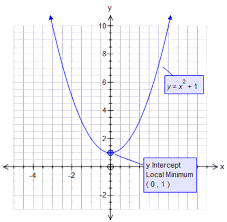
\includegraphics[width=0.35\textwidth]{x^2 + 1.png}
        \caption{Graph of \( y = x^2 + 1 \).}
        \label{fig:sample_image}
    \end{figure}
    Notice that
    \begin{equation*}
    \begin{aligned}
    y &= x^2 + 1 \\
    \implies 0 &\geq (-2)^2 + 1 \\
    \implies 0 &\geq 5 \text{, which is not true.}
    \end{aligned}
    \end{equation*}
    Then, notice that
    \begin{equation*}
    \begin{aligned}
    2 &\geq 0^2 + 1 \\
    \implies 2 &\geq 1 \text{, which is true!}
    \end{aligned}
    \end{equation*}
    Here is the region being considered:
    \begin{figure}[H]
        \centering
        
\includegraphics[width=0.35\textwidth]{sample_image.jpg}
        \caption{Sample image illustrating the concept.}
        \label{fig:sample_image}
    \end{figure}
\end{solutionbox}
\end{examplebox}

\section*{Ellipse}
\begin{definitionbox}
The equation of an ellipse is defined by
\[
    \dfrac{(x - h)^2}{a^2} + \dfrac{(y - k)^2}{b^2} = 1 \text{.}
\]
\begin{notebox}
Recall the equation of the circle, which is based on the equation of the ellipse when \( a = b = 1 \):
\[
    \text{Circle:} \quad (x - h)^2 + (y - k)^2 = r^2 \text{,}
\]
where \( (h, k) \) is the centre, \( a \) represents the \( x \)-axis radius, and \( b \) represents the \( y \)-axis radius.
\end{notebox}
\end{definitionbox}

\section*{Example of Skecthing an Ellipse}
\begin{examplebox}
Sketch the region of the set defined by
\[
    A = \{ (x, y) \mid x^2 + 4y^2 > 4 \} \text{.}
\]
\begin{solutionbox}
    Notice that
    \[
        x^2 + 4y^2 = 4 \text{.}
    \]
    This means the centre is at \( (0, 0) \).
    Also,
    \[
        \dfrac{x^2}{4} + \dfrac{y^2}{1} = 1
    \]
    provides that the \( x \)-axis radius is \( a = 2 \) and the \( y \)-axis radius is \( b = 1 \). \\
    \\
    Here is the corresponding illustration:
    \\\textbf{self-note: add the illustratoin from the lecture note from your camera roll}
    \begin{figure}[H]
        \centering
        
\includegraphics[width=0.35\textwidth]{sample_image.jpg}
        \caption{Illustration of ellipse.}
        \label{fig:sample_image}
    \end{figure}
    \begin{notebox}
    Note that dashed lines are used to denote that the edge of the ellipse is \textbf{not included} in the region \( A \).
    \end{notebox}
    Check the point \( (0, 0) \):
    \[
        0^2 + 4 \cdot 0^2 > 4
    \]
    \[
        \implies 0 > 4 \text{,}
    \]
    which is not true. \\
    \\
    Therefore, the inside of the ellipse is \textbf{not} to be shaded in. \\
    \\
    Check the point \( (3, 0) \) :
    \[
        3^2 + 4 \cdot 0^2 > 4
    \]
    \[
        \implies 9 > 4 \text{,}
    \]
    which is true. \\
    \\
    This means, the outer region (excluding the edge) of the ellipse is the region of interest as denoted by \( A \).
\end{solutionbox}
\end{examplebox}

\section*{Introducing the Hyperbola}
\begin{definitionbox}
The equation of a hyperbola is defined by
\[
    \dfrac{x^2}{a^2} - \dfrac{y^2}{b^2} = 1
\]
\begin{illustrationbox}
    \textbf{self-note: add the image of the corresponding illustration here (see the lecture note)}
    \begin{figure}[H]
        \centering
        
\includegraphics[width=0.35\textwidth]{sample_image.jpg}
        \caption{Sample image illustrating the concept.}
        \label{fig:sample_image}
    \end{figure}
\end{illustrationbox}
\[
    \dfrac{y^2}{b^2} - \dfrac{x^2}{a^2} = 1
\]
\begin{illustrationbox}
    \textbf{self-note: add the image of the corresponding illustration here (see the lecture note)}
    \begin{figure}[H]
        \centering
        
\includegraphics[width=0.35\textwidth]{sample_image.jpg}
        \caption{Sample image illustrating the concept.}
        \label{fig:sample_image}
    \end{figure}
\end{illustrationbox}
\end{definitionbox}

\section*{Welcome to Linear Algebra...}
\subsection*{well... not really!}

\section*{Section 2.1/2.2: Welcome to 3D Space!}
\begin{remarkbox}
Recall that the cartesian coordinate system considers the 2-dimensional realm: a system in \( \mathbb{R}^2 \).
\begin{illustrationbox}
    \textbf{self-note: add the cartesian plane — the typical one in 2D}
    \begin{figure}[H]
        \centering
        
\includegraphics[width=0.35\textwidth]{sample_image.jpg}
        \caption{Sample image illustrating the concept.}
        \label{fig:sample_image}
    \end{figure}
\end{illustrationbox}
Now, check out the cartesian coordinate system being introduced in MAT232, considering the 3-dimensional realm; \( \mathbb{R}^3 \):
\begin{illustrationbox}
    \textbf{self-note: add the illustration for the 3D cartesian plane, the z-axis in addition to the x- and \( y \)-axis}.
    \begin{figure}[H]
        \centering
        
\includegraphics[width=0.35\textwidth]{sample_image.jpg}
        \caption{Sample image illustrating the concept.}
        \label{fig:sample_image}
    \end{figure}
\end{illustrationbox}
\end{remarkbox}

\begin{notebox}
\underline{In 2D:} \\
Notice that \( \mathbb{R}^2 = \mathbb{R} \times \mathbb{R} \), where the first \( \mathbb{R} \) represents the \( x \)-values and the second \( \mathbb{R} \) represents the \( y \)-values.
\\
\underline{Now, in 3D:} \\
Notice that \( \mathbb{R}^3 = \mathbb{R} \times \mathbb{R} \times \mathbb{R} \).
\begin{itemize}
    \item The first \( \mathbb{R} \) represents the \( x \)-values;
    \item The second \( \mathbb{R} \) represents the \( y \)-values;
    \item The third \( \mathbb{R} \) represents the \( z \)-values.
\end{itemize}
\end{notebox}

\section*{Example of Plotting in a 3D Cartesian Plane}
\begin{examplebox}
Plot the points \( (-1, 2, -3) \) and \( (2, -4, 2) \).
\begin{illustrationbox}
    \textbf{self-note: add the illustration here!!}
    \begin{figure}[H]
        \centering
        
\includegraphics[width=0.35\textwidth]{sample_image.jpg}
        \caption{Sample image illustrating the concept.}
        \label{fig:sample_image}
    \end{figure}
\end{illustrationbox}
\textit{Follow the line segments denoted in \textbf{purple} for an interpretation guide of how the three components contribute to the final point destination, for \( (-1, 2, -3) \).} \\
\textit{Follow the line segments denoted in \textbf{green} for an interpretation guide of how the three components contribute to the final point destination, for \( (2, -4, 2) \).} \\
\end{examplebox}

\section*{Interpreting Planes}
\begin{conceptbox}
Notice that in a 2D world, there is no notion of height when considering the \( x, y \)-plane. In a 3D world, \( z = 0 \). \\
\\
Now, have a look at the basic planes for a 3D cartesian graph: \\
\\
\underline{The \( xy \) plane:}
\[
    x = 0 \quad\quad\quad (x, y, 0)
\]
\begin{figure}[H]
    \centering
    
\includegraphics[width=0.35\textwidth]{sample_image.jpg}
    \caption{Sample image illustrating the concept.}
    \label{fig:sample_image}
\end{figure}
\underline{The \( yz \) plane:}
\[
    x = 0 \quad\quad\quad (0, y, z)
\]
\begin{figure}[H]
    \centering
    
\includegraphics[width=0.35\textwidth]{sample_image.jpg}
    \caption{Sample image illustrating the concept.}
    \label{fig:sample_image}
\end{figure}
\underline{The \( xz \) plane:}
\[
    x = 0 \quad\quad\quad (x, 0, z)
\]
\begin{figure}[H]
    \centering
    
\includegraphics[width=0.35\textwidth]{sample_image.jpg}
    \caption{Sample image illustrating the concept.}
    \label{fig:sample_image}
\end{figure}
\end{conceptbox}

\section*{Let's Try Going from 2D to 3D}
\begin{examplebox}
Consider the graph defined by \( y = 2 \) on a 2D cartesian graph:
\begin{figure}[H]
    \centering
    
\includegraphics[width=0.35\textwidth]{sample_image.jpg}
    \caption{Sample image illustrating the concept.}
    \label{fig:sample_image}
\end{figure}
Here's how that would look like in a 3D cartesian space:
\begin{figure}[H]
    \centering
    
\includegraphics[width=0.35\textwidth]{sample_image.jpg}
    \caption{Sample image illustrating the concept.}
    \label{fig:sample_image}
\end{figure}
\end{examplebox}

\begin{examplebox}
Consider the graph of a circle defined by
\[
    x^2 + y^2 = 4 \text{.}
\]
\begin{figure}[H]
    \centering
    
\includegraphics[width=0.35\textwidth]{sample_image.jpg}
    \caption{Sample image illustrating the concept.}
    \label{fig:sample_image}
\end{figure}
If this circle is brought to the 3D world, stretched along the \( z \)-axis, for any values of \( z \), then a cylinder is created (the cirle is the cross-section shape).
\begin{figure}[H]
    \centering
    
\includegraphics[width=0.35\textwidth]{sample_image.jpg}
    \caption{Sample image illustrating the concept.}
    \label{fig:sample_image}
\end{figure}
\end{examplebox}

\subsection*{Next Lecture: We Discuss Vectors!}

\section*{Lecture Title}
\begin{notebox}
This template is designed for MAT232 lecture notes. Replace this content with your specific lecture details.
\end{notebox}

\section*{Key Concepts}
\begin{definitionbox}
A \textbf{parametric equation} is a set of equations that express the coordinates of the points of a curve as functions of a variable, called a parameter.
\end{definitionbox}

\section*{Examples}
\begin{examplebox}
\textbf{Example 1:} Consider the parametric equations:
\[ x = t, \quad y = t^2, \quad t \in \mathbb{R}. \]
\begin{itemize}
    \item At $t = 0$, $(x, y) = (0, 0)$.
    \item At $t = 1$, $(x, y) = (1, 1)$.
\end{itemize}
This describes a parabola.

\begin{figure}[H]
    \centering
    
\includegraphics[width=0.35\textwidth]{sample_image.jpg}
    \caption{Sample image illustrating the concept.}
    \label{fig:sample_image}
\end{figure}

\end{examplebox}

\section*{Theorems and Proofs}
\begin{theorembox}
\textbf{Theorem:} If $x(t)$ and $y(t)$ are differentiable functions, the slope of the curve is given by:
\[ \frac{dy}{dx} = \frac{\frac{dy}{dt}}{\frac{dx}{dt}}, \quad \text{provided } \frac{dx}{dt} \neq 0. \]

\begin{figure}[H]
    \centering
    
\includegraphics[width=0.35\textwidth]{sample_image1.jpg}
    \caption{Graphical representation of the theorem.}
    \label{fig:sample_image1}
\end{figure}

\end{theorembox}

\section*{Additional Notes}
\begin{notebox}
Always check the domain of the parameter $t$ when solving problems involving parametric equations.
\end{notebox}

\end{document}
